\documentclass{ctexart}
\usepackage[margin=1in]{geometry}
\usepackage{graphicx}
\begin{document}
\section{密封}
\subsection{静密封}
\paragraph{}根据功能要求本文所设计水下机器人的最大作业深度为500米,耐压舱在水下需承受的压力载荷为5MPa,根据压力容器设计规范,在对压力容器设计时,其试验压力应为设计压力的1.5倍,这样才能保证所设计容器的可靠性,故本文取整定义8MPa为该耐压舱的试验压力。考虑本文所设计水下机器人的工作性质,安全系数定为1.5。
\paragraph{}水下机器人耐压壳体内部通常装有电子部件、检测仪器等。为了方便检修和拆卸内部元件,耐压壳体必须有一个可拆卸的封头。可拆卸封头与壳体配合表面之间存在间隙(结构的需要、加工误差、光洁度),而且间隙会随着连接件受压变形、表面磨损等原因变化。要阻止海水进入,需将已有间隙塞满,具备密封能力。
\paragraph{}水下机器人耐压舱除了要满足在最大作业深度下的强度及稳定性之外,还应保证在该设计压力下不发生泄漏。由于耐压舱内装有主控制电路板及各类传感器等价值不菲的核心元件,一旦发生泄漏将会使整个水下机器人陷入瘫痪状态,内部元件也将全部失灵,从而产生巨大的经济损失,甚至致使整机在水下无法找回,发生核心技术外泄的风险,故耐压舱壳体与封头拥有良好的密封性也是极其重要的。耐压舱的密封类别为静密封,密封形式为活塞式双道径向密封。由于壳体封头口内壁不易加工,故在封头套筒外壁处添加密封槽。密封圈装于密封槽内,封头套筒与壳体封头口内壁采用间隙配合,且通过设置配合公差使封头套筒外径略小于壳体封头口内径。安装完成后,O型密封圈受到壳体封头口内壁挤压变形,并通过摩擦力使封头与壳体稳固连接,同时堵住配合间隙,从而达到密封效果。
\paragraph{}对于密封件采用的是O型密封圈。O型密封圈以其截面形状为O形而得名,是最常见及用途最广的密封件之一,通常置于密封槽中进行密封,其价格低廉、来源广泛、体积小、拆装简易、寿命高、可靠性好,且同时适用于动、静密封,故O型密封圈常被用于水下机器人的舱体密封。O型密封圈材料的选取通常需考虑其强度、硬度、刚度、弹性及疲劳强度等力学性能,在正常承压时容易产生不可逆形变、寿命过短及压入密封间隙等情况而导致密封失效,如表所示几种O型密封圈材料的性能: 
\begin{tabular}{|c|c|c|c|c|}
    \hline
    材料种类&优点&缺点&用途 & 使用温度$(^\circ C)$ \\
    \hline
    丁腈橡胶&耐磨、耐热、柔性好&耐电、臭氧性差&密封件、耐油管、隔膜&-50\~{}110 \\
    \hline
    硅橡胶&耐热、耐老化&价格高、强度差&隔膜、减震器&-60\~{}250 \\
    \hline
    氟硅橡胶&耐热、耐寒&强度差&橡胶管、垫圈、密封件&-55\~{}200 \\
    \hline
    氟醇橡胶&耐油、耐寒&耐水、耐磨性差&胶管、减震材料、密封制品&-55\~{}110 \\
    \hline
\end{tabular}
\paragraph{}综合上述O型密封圈材料性能情况及各前人的设计经验,本文采用的O型密封圈的材料为丁腈橡胶。O型密封圈具有良好的记忆挤压特性,当其受压时由于橡胶材料的特性会使其向着原始状态或形态进行恢复,从而紧贴于密封接触面实现密封。在密封时O型橡胶密封圈基于其良好的流动性而补偿密封接触面的设计配合公差,填满密封接触面的间隙或不平,实现稳定密封。在静密封中,O型密封圈的密封效果几乎可实现零泄漏。就O型密封的最大压缩量的选取而言常用下式来表示:
\[W=\frac{d_0-s}{d_0}\times 100\%     \]
式中,$d_0$表示O型密封圈截面直径;$s$表示密封槽深度。根据项目标准,本文所设计压缩率为$18\%$。
\paragraph{}对于密封槽的截面形状,其选用情况如表所示:\\ 
\begin{tabular}{|c|c|c|}
    \hline
    密封槽截面形状&名称&适用场合 \\
    \hline
    矩形&矩形密封槽&同时适用于动、静密封 \\
    \hline
    V形&V型密封槽&只适用于固定密封 \\
    \hline
    半圆形&半圆形密封槽&可用于旋转密封,但很少用 \\
    \hline
    梯形&梯形密封槽&用于摩擦力要求较低的场合 \\
    \hline
    三角形&三角形密封槽&适用于固定密封 \\
    \hline
\end{tabular}
\paragraph{}本文耐压舱的密封类别为静密封,且作业环境为非高压环境,故密封槽选用的是最常见的矩形密封槽。
            根据国家标准,密封槽的槽棱及槽底倒角的设计范围分别为0.1~0.3mm及0.2~0.4mm,故结合参考产品的设计经验,
            本文密封槽的槽棱及槽底的倒角均为0.2mm。
\paragraph{}在结构未进行工作的转态下,外界压力可以近似为零,此时密封圈装入密封槽内,由于受到壳体挤压的初始预压力而产生径向压缩变形,
            从而实现密封;当结构处于低压环境下,由于外部水压的作用,O型圈紧贴壳体内壁及密封槽堵住密封间隙;当水压增大至较高压力,即参考压力为9.8兆帕时,
            O型圈部分挤入密封间隙。根据本文的AUV工作环境压力为5兆帕可知,O型圈可以正常工作。
\paragraph{}综上所述,本文选择套筒式的装配方式及O型密封圈来实现耐压舱封头与壳体的连接及密封。封头端面的水密接插孔用于接入水密插件,
            除了能密封封头端面之外,还能实现壳体内部核心元件与外部元件的能源与信号传输。
\subsection{水下推进器的旋转动密封}
\paragraph{}动密封是由一对或几对平面接触的密封环在流体压力与补偿机构弹力的作用下以一定压力保持贴合,并相对滑动形成一个动密封装置。
            一般情况下, 动密封主要用于压缩机、泵等机械设备上转轴上的密封, 主要由动环、静环、密封圈、弹簧、推环、弹簧座、螺钉等部件组成, 具有一定的复杂性。在补偿机构弹力 (或磁力) 和流体压力的作用下,
             至少有一对垂直于旋转轴线的端面在辅助密封的配合下, 保持着贴合状态并相对活动以防止流体泄露的装置。其效果图如下:\\
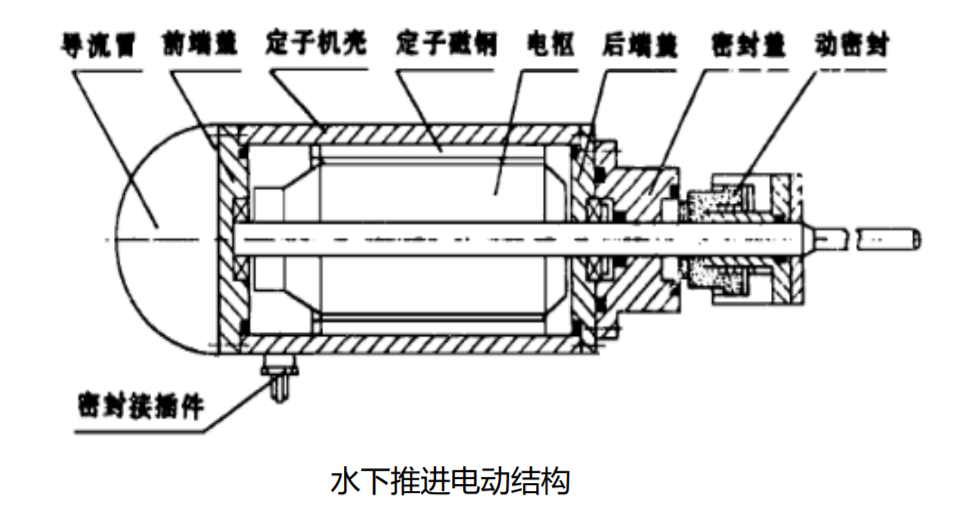
\includegraphics[scale=0.4]{./mifeng.png}
            
\paragraph{}综上所述,在水下推进系统中,我们采用了利用带补偿环的旋转动密封的密封形式,密封位置与密封装置结构如图所示。旋转机械动密封安装在旋转轴上,密封腔内有传动座、弹簧、推环、动环、动环密封圈,它们随轴一起旋转。
            其他零件,包括静环、静环密封圈和垫片安装在压盖内,压盖与密封腔体用螺栓连接。轴通过传动座、弹簧带动环旋转,而静环则静止于压盖内。动环在弹簧力和水压力的作用下,与静环的端面紧密贴合,并发生相对滑动,
            阻止了海水沿端面间的径向泄漏。在相对运动中接触面(摩擦副)磨损后会在弹簧和密封海水压力的推动下实现补偿,始终保持两个密封端面的紧密接触。动环密封圈阻止了外界水可能沿动环与轴之间的间隙处泄漏;而静环密封圈会阻止海水可能沿静环与端盖之间的间隙处泄漏。


\paragraph{}

\end{document}